\section{25.11.2014 - Flip-Flop}

In questa esperienza studieremo il funzionamento dei Flip-Flop e di alcuni circuiti costruiti con essi.

\subsection*{Strumenti e materiali}

\begin{itemize} [noitemsep]
	\item Oscilloscopio Agilent DSO-X 2002A (bandwidth \SI{70}{\mega\hertz}, sample rate \num{2} GSa/s);
	\item Generatore di tensione continua Agilent E3631A (max $\pm \, \SI{25}{\volt}$ o $\pm \, \SI{6}{\volt}$);
	\item Multimetro Agilent 34410A a sei cifre e mezza;
	\item Un integrato 7400, composto di quattro porte logiche TTL NAND; % '00;
	\item Un integrato 74LS02, composto di quattro porte logiche NOR;
	\item Un integrato LS109;
	%\item Un integrato 74LS125, composto di quattro porte logiche buffer TTL 3State;
	\item Basetta a LED;		
	\item Resistenze e capacità di vari valori;
	\item Breadboard e cablaggi vari.
\end{itemize}

\subsection{Flip-Flop SR}

\subsubsection*{FF SR con porte NAND tipo latch}

%\begin{wrapfigure}[12]{r}{0.45\textwidth}
%	\centering
%	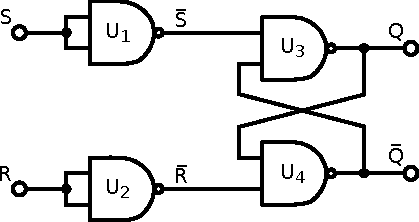
\includegraphics[width=.35\textwidth]{../E11/latex/FF-SR-async.pdf}
%	\caption{Schema circuitale del \textit{flip-flop} SR asincrono}
%	\label{cir11:FF-SR-a}
%\end{wrapfigure}

In questa prima parte dell'esperienza abbiamo construito il FF SR utilizzando delle porte NAND.
Il circuito è riportato in Figura \ref{cir11:FF-SR-a} e, come gli altri circuiti logici, il funzionamento è stato verificato con la basetta a LED.

Analizziamo ora il circuito logico.
U1 e U2 sono delle porte NAND le cui entrate sono allo stesso potenziale, dunque sono due NOT rispettivamente per i segnali S ed R (terza e quarta colonna della tabella sottostante).

Ad esempio, poniamo S ed R ad 1 logico: quindi U1 e U2 li renderanno degli 0 logici; dunque, considerando U3 ed U4 come interruttori, se hanno uno degli ingressi a 0 l'uscita sarà sempre 1 indipendentemente dall'altra entrata.
Questo stato è poco interessante dal punto di vista logico (non ho due uscite una la negazione dell'altra), quindi cercheremo di evitarlo.

Se invece pongo entrambi gli ingressi di U3 e U4 ad 1 logico (cioè con S=R=0 logico), questi mi restituiranno 1 se l'altro ingresso sarà 0, altrimenti 1.
Ciò ovviamente rende le uscite dipendenti dalle tensioni presenti prima del cambiamento di S e di R, rendendolo indeterminate (nel senso che, se non sapessimo i valori di $Q$ e $\bar Q$, a priori non potremmo stabilire, ponendo S=R=0, quale sarà l'uscita).
Sfrutteremo questa indeterminazione come elemento di memoria per conservare la nostra informazione fino alla scrittura successiva, che può essere effettuata ponendo S ed R a valori l'uno la negazione dell'altro.

La tabella di verità del circuito logico è la seguente, con $Q_n$ la tensione ad un ciclo e $Q_{n+1}$ quella al ciclo successivo\footnote{In realtà per poter parlare di un ciclo dovremmo attendere la presenza di un attivatore, che se posto come onda quadra ad una certa frequenza può fornirci un clock.
Ciò sarà presente nel circuito successivo.}.

\begin{savenotes}
\begin{figure}[htpc]
\centering
	\begin{subfigure}[hc]{.4\textwidth}
		\centering
		{\renewcommand{\arraystretch}{1.1}%
		\begin{tabular}{|c|c|c|c|c|c|}
		\hline
		S & R & $\bar S$ & $\bar R$ & $Q_{n+1}$ & $\bar Q_{n+1}$ \\
		\hline \hline
		0 & 0 & 1 & 1 & $Q_n$ & $\bar Q_n$\\
		\hline
		0 & 1 & 1 & 0 &  0  &  1\\
		\hline
		1 & 0 & 0 & 1 &  1  &  0\\
		\hline
		1 & 1 & 0 & 0 & ? & ?\\
		\hline
		\end{tabular}}
		\label{tab11:FFSR}
        \end{subfigure}
        \begin{subfigure}[hc]{.4\textwidth}
		\centering
		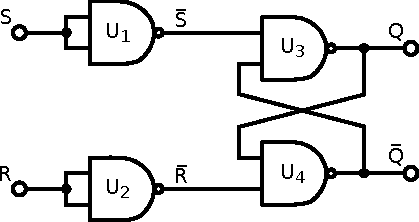
\includegraphics[width=.7\textwidth]{../E11/latex/FF-SR-async.pdf}
		\caption{}
		\label{cir11:FF-SR-a}
        \end{subfigure}
\caption{Tabella di verità e schema circuitale del \textit{flip-flop} SR asincrono.}
\end{figure}
\end{savenotes}

Per verificarne il funzionamento, abbiamo collegato entrambe le uscite del Flip-Flop alla basetta al led.
Abbiamo notato che non avevamo mai due led accessi contemporaneamente, eccetto nel caso in cui sia Set che Reset erano ad 1 logico, confermando la correttezza della nostra analisi circuitale.

\subsubsection*{FF SR con Clock}

%\begin{wrapfigure}[13]{r}{0.45\textwidth}
%	\centering
%	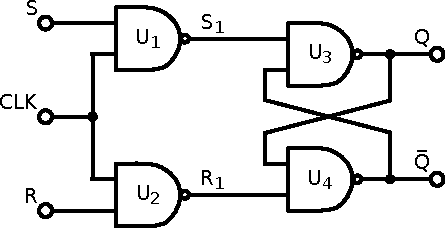
\includegraphics[width=.35\textwidth]{../E11/latex/FF-SR-sync.pdf}
%	\caption{Schema circuitale del \textit{flip-flop} SR sincrono}
%	\label{cir11:FF-SR-s}
%\end{wrapfigure}

In questo secondo circuito vogliamo rendere sincrono quello precedente, inserendo un attivatore (CLK nella tabella sottostante) che possa bloccare eventuali cambiamenti in uscita (cioè la porti in modalità di memoria) indipendentemente da S ed R, come nel circuito in Figura \ref{cir11:FF-SR-s}.
Portando come segnale dell'attivatore una forma d'onda quadra potremmo anche creare un clock.
La tabella di verità può essere ricavata con considerazioni analoghe al paragrafo precedente, ed è quella sottostante

\begin{figure}[htpc]
\centering
	\begin{subfigure}[hc]{.4\textwidth}
		\centering
		{\renewcommand{\arraystretch}{1.2}%
		\begin{tabular}{|c||c|c|c|c|}
		\hline
		CLK & S & R & $Q_{n+1}$ & $\bar Q_{n+1}$  \\
		\hline \hline
		0 & X & X & $Q_n$ & $\bar Q_n$\\
		\hline \hline
		 1&0 & 0 & $Q_n$ & $\bar Q_n$\\
		\hline
		1&0 & 1 & 0 &1\\
		\hline
		1&1 & 0 & 1 & 0\\
		\hline
		1&1 & 1 & ? & ?\\
		\hline
		\end{tabular}}
		\caption{}
		\label{tab11:FFSR2}
        \end{subfigure}
        \begin{subfigure}[hc]{.4\textwidth}
		\centering
		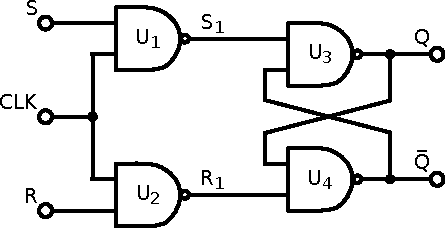
\includegraphics[width=.7\textwidth]{../E11/latex/FF-SR-sync.pdf}
		\caption{}
		\label{cir11:FF-SR-s}
        \end{subfigure}
\caption{Tabella di verità e schema circuitale del \textit{flip-flop} SR sincrono.}
\end{figure}

Notiamo inoltre che anche in questo caso, se sia S che R sono ad 1 logico, le uscite non sono utili per un utilizzo in circuiti logici.

\subsubsection*{Latch tipo D}

Cerchiamo ora di risolvere il problema della presenza dello stato indesiderato dato da S=R=0 logico.
Un modo semplice per evitare che possa accadere è di utilizzare il circuito riportato in Figura \ref{cir11:D-type-latch} assieme alla sua tabella di verità.

\begin{figure}[htpc]
\centering
	\begin{subfigure}[hc]{.4\textwidth}
		\centering
		{\renewcommand{\arraystretch}{1.2}%
		\begin{tabular}{|c|c|c|c|}
		\hline
		D & CLK	& $Q_{n+1}$	& $\bar Q_{n+1}$  \\
		\hline
		X & 0   & $Q_n$		& $\bar Q_n$\\
		\hline
		1 & 1   & 1		& 0\\
		\hline
		0 & 1   & 0		& 1\\
		\hline
		\end{tabular}}
		\caption{}
		\label{tab11:Latch_D}
        \end{subfigure}
        \begin{subfigure}[hc]{.4\textwidth}
		\centering
		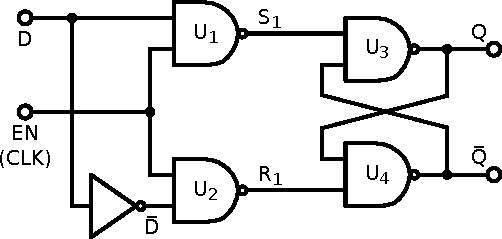
\includegraphics[width=.7\textwidth]{../E11/latex/D-type-latch.pdf}
		\caption{}
		\label{cir11:D-type-latch}
        \end{subfigure}
\caption{Tabella di verità e schema circuitale del D-Type Latch.}
\end{figure}

Abbiamo inoltre notato che, con CLK ad 1, lasciando l'ingresso D flottante l'uscita Q era bassa.
Ciò è in contraddizione con le porte integrate, in quanto quando un ingresso non è collegato a nessun riferimento viene visto come alto.
Abbiamo capito che ciò era dovuto al fatto che abbiamo collegato il cavo dati alla basetta al led per vedere quando esso era a 0 o 1 logico.
La basetta al led è costruita con resistenze di pull-down così che quando il segnale in ingresso è basso i led sono spenti.
Dunque se monitoriamo il segnale D con la basetta, esso è collegato con resistenze di pull-down a comune.
Abbiamo infatti verificato che scollegandolo dalla basetta, l'ingresso D flottante causava un uscita Q alta.

\subsubsection*{FF SR con porte NOR}

Abbiamo provato a realizzare un FF SR con porte NOR.
Il principio di funzionamento è lo stesso di quello costruito utilizzando porte NAND.
L'unica differenza sta nel fatto che il circuito si trova in memoria quando sia S che R sono a 0 logico.
Lo schema circuitale elaborato è riportato nella seguente figura.

\begin{figure}[htpc]
\centering
        \begin{subfigure}[hc]{.5\textwidth}
		\centering
		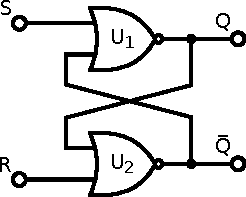
\includegraphics[width=.35\textwidth]{../E11/latex/FF-w-NOR.pdf}
		\caption{}
		\label{cir11:nor}
        \end{subfigure}
	\begin{subfigure}[hc]{.4\textwidth}
		\centering
		{\renewcommand{\arraystretch}{1.1}%
		\begin{tabular}{|c|c|c|c|}
		\hline
		S & R & $Q_{n+1}$ & $\bar Q_{n+1}$  \\
		\hline
		1 & 1  & ?&?\\
		\hline
		1&0 & 1 & 0\\
		\hline
		0&1 & 0  &1\\
		\hline
		0&0 & $Q_n$ & $\bar Q_n$\\
		\hline
		\end{tabular}}
		\caption{}
		\label{tab11:nor}
        \end{subfigure}
\caption{Tabella di verità e schema circuitale di un FF SR composto di porte NOR}
\end{figure}

Per completezza riportiamo anche la tabella di verità del circuito.
Il circuito, come sempre, è stato verificato utilizzado la basetta a led.

\subsection{Interruttori e circuiti anti-rimbalzo}

\begin{figure}[htpc]
\centering
        \begin{subfigure}[hc]{.3\textwidth}
		\centering
		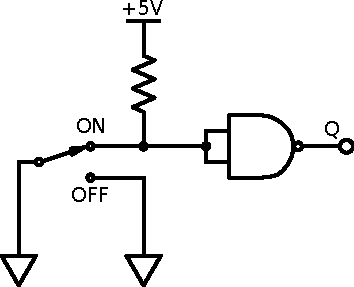
\includegraphics[width=.7\textwidth]{../E11/latex/rimbalzo.pdf}
		\caption{}
		\label{cir11:rimb}
        \end{subfigure}
	\begin{subfigure}[hc]{.3\textwidth}
		\centering
		{\renewcommand{\arraystretch}{1.2}%
		\begin{tabular}{|c|c|c|c|}
		\hline
		$\bar S$ & $\bar R$ & $Q_{n+1}$ & $\bar Q_{n+1}$  \\
		\hline
		0 & 0  & ?&?\\
		\hline
		0&1 & 1 & 0\\
		\hline
		1&0 & 0  &1\\
		\hline
		1&1 & $Q_n$ & $\bar Q_n$\\
		\hline
		\end{tabular}}
		\caption{}
		\label{tab11:antirimb}
        \end{subfigure}
        \begin{subfigure}[hc]{.3\textwidth}
		\centering
		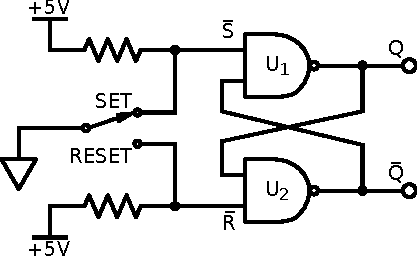
\includegraphics[width=.9\textwidth]{../E11/latex/anti-rimbalzo.pdf}
		\caption{}
		\label{cir11:no-rimb}
        \end{subfigure}
\caption{Schema circuitale di un interruttore semplice, tabella di verità e schema circuitale di un interruttore anti-rimbalzo.}
\end{figure}

%\begin{wrapfigure}[14]{l}{0.45\textwidth}
%\centering
%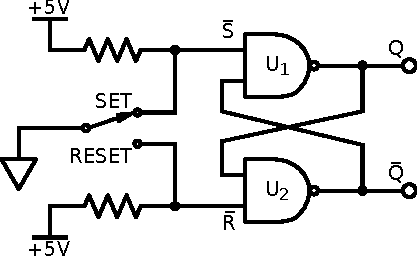
\includegraphics[width=.25\textwidth]{../E11/latex/anti-rimbalzo.pdf}
%\caption{.}
%\label{cir11:no-rimb}
%\end{wrapfigure}

Un problema degli interruttori è quello del rimbalzo.
Infatti lo switch meccanico dell'interruttore non è istantaneo in quanto composto da una linguetta conduttrice che fa da contatto.
Nel momento in cui la linguetta passa da un contatto all'altro abbiamo dei rimbalzi di tensione.
Un modo per risolvere questo problema è quello di utilizzare un interruttore a transistor oppure inserire appena dopo l'interruttore meccanico un circuito di anti-rimbalzo.
Lo schema è riportato in Figura \ref{cir11:no-rimb}.
Tale circuito ci permette di evitare i rimbalzi poichè quando la linguetta è scollegata sia dal SET che dal RESET abbiamo il circuito in configurazione memoria.
Ciò è dovuto al fatto che abbiamo inserito delle resistenze di \textit{pull-up} che portano gli ingressi delle NAND a 1 logico.

Dopo averne studiato le caratteristiche dal punto di vista teorico, ne abbiamo verificato il funzionamento sperimentalmente.
I risultati sono riportati nei seguenti grafici.

\begin{figure}[htpc]
\centering
	\begin{subfigure}[hc]{.49\textwidth}
		\centering
		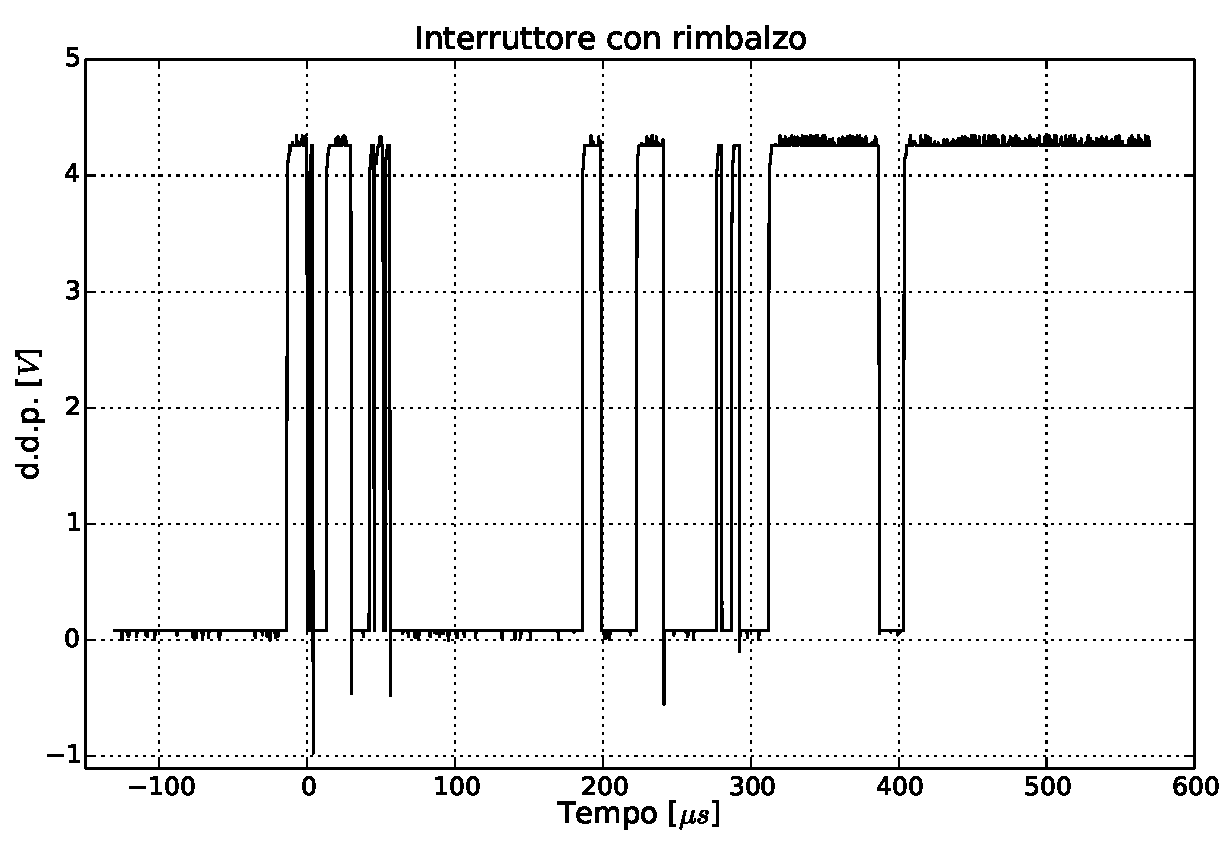
\includegraphics[width=.99\textwidth]{../E11/latex/rimb.pdf}
		\caption{}
		\label{gr11:rimb}
        \end{subfigure}%
        \begin{subfigure}[hc]{.49\textwidth}
		\centering
		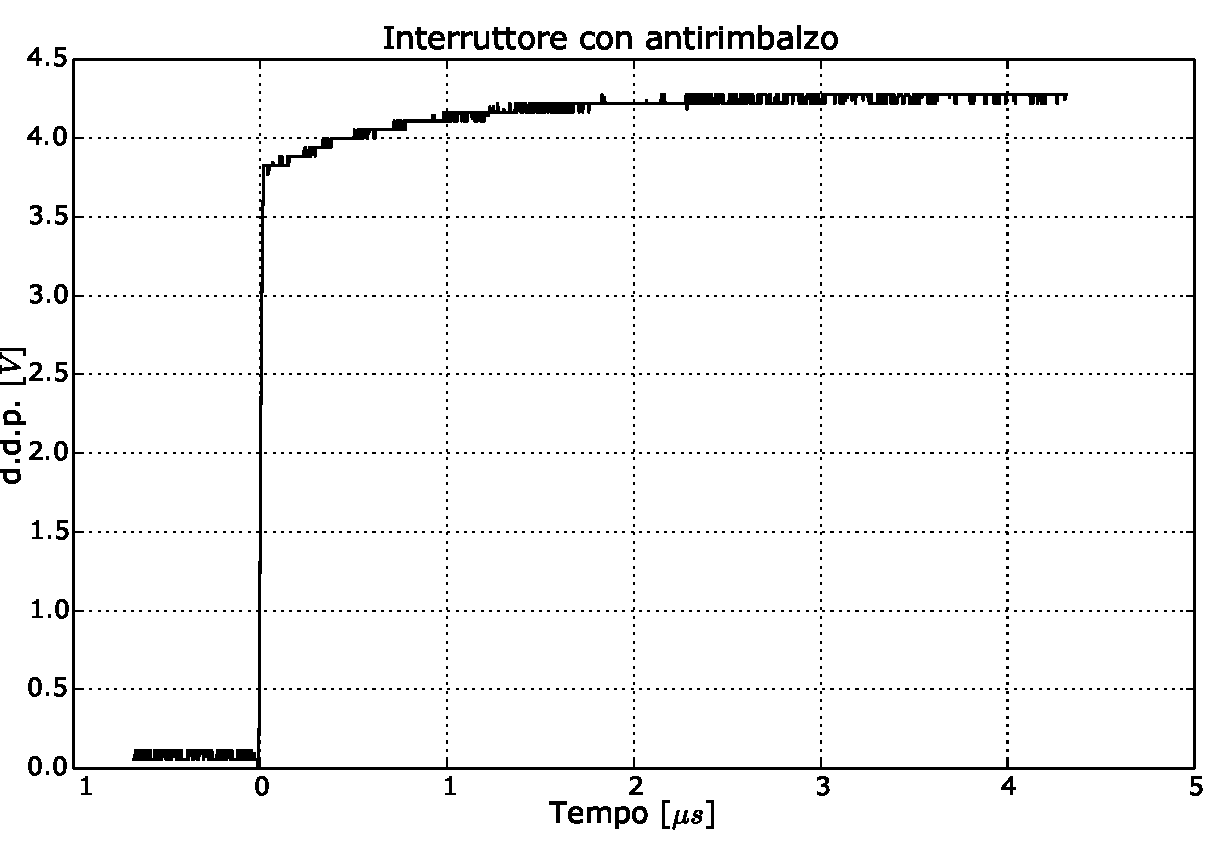
\includegraphics[width=.99\textwidth]{../E11/latex/antirimb.pdf}
		\caption{}
		\label{gr11:no-rimb}
        \end{subfigure}
\caption{I due grafici riportano il comportamento degli interruttori: quello a sinistra è un interruttore semplice, quello a destra è un interruttore seguito da un circuito antirimbalzo.}
\end{figure}


Come vediamo, il tempo di rimbalzo senza correzione è di circa \SI{4}{\milli\second}.
Utilizzando il circuito FF, invece, abbiamo completamente eliminato il problema.
La forma d'onda in uscita non è perfettamente a scalino in quanto i generatori di corrente non sono ideali e le impedenze non sono ottimizzate.

\subsubsection*{Comandi separati Marcia/Arresto}

\begin{figure}[H]
%\begin{wrapfigure}[14]{r}{0.45\textwidth}
	\centering
	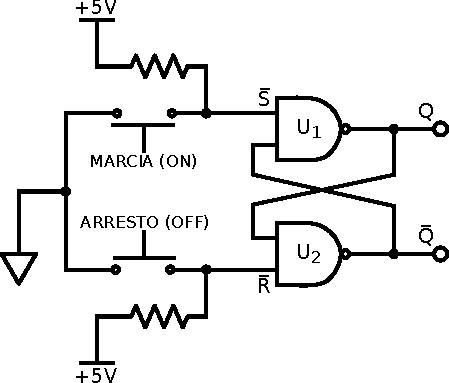
\includegraphics[width=.25\textwidth]{../E11/latex/motorefermo.pdf}
	\caption{Schema del circuito di comando di \textit{marcia/arresto}.}
	\label{cir11:marcia}
%\end{wrapfigure}
\end{figure}

Possiamo apportare delle utili modifiche al circuito anti-rimbalzo separando il comando Marcia/Arresto.
Così facendo possiamo avere un circuito che può essere messo nella condizione di memoria.
Il circuito è riportato in fugura (\ref{cir11:marcia}).

Dobbiamo ricordarci di non mettere mai contemporaneamente a 0 logico sia Marcia che Arresto in quanto avremmo una condizione di indeterminazione che ovviamente non vogliamo.

\subsection{Divisore di frequenze}



Come ultima parte dell'esperienza abbiamo realizzato un divisore di frequenze servendoci dell'integrato 74LS109, che contiene 2 FF di tipo JK.
I FF di tipo JK opportunamente alimentati diventano dei FF di tipo T (Toggle).

\begin{wrapfigure}[11]{r}{0.45\textwidth}
	\centering
	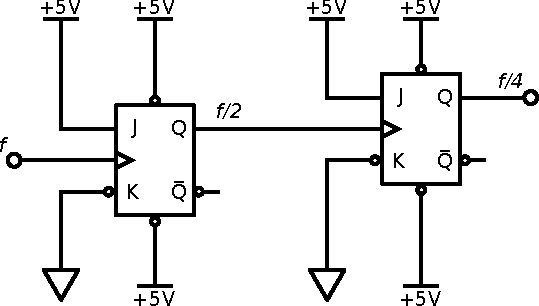
\includegraphics[width=.30\textwidth]{../E11/latex/frequency-divider.pdf}
	\caption{Schema circuitale del divisore di frequenza.}
	\label{cir11:freq-div}
\end{wrapfigure}

Essi permettono di fare una divisione di frequenze per multipli di 2 e, tramite circuiti leggermente più complicati anche per altri numeri coprimi di 2.



Osservando il circuito riportato in Figura \ref{cir11:freq-div}, possiamo notare che il clock del secondo FF è comandato dal dato del primo $D_1$.
Poiché $J_1$ è sempre a 1, $D_1$ cambierà di stato solo ad ogni fronte di salita del clock.
Questo ragionamento è lo stesso anche per il secondo FF e pertanto, ogni FF impostato in questo modo produce in uscita un'onda quadra di frequenza dimezzata rispetto al clock che riceve.

\begin{figure}[H]
\centering
	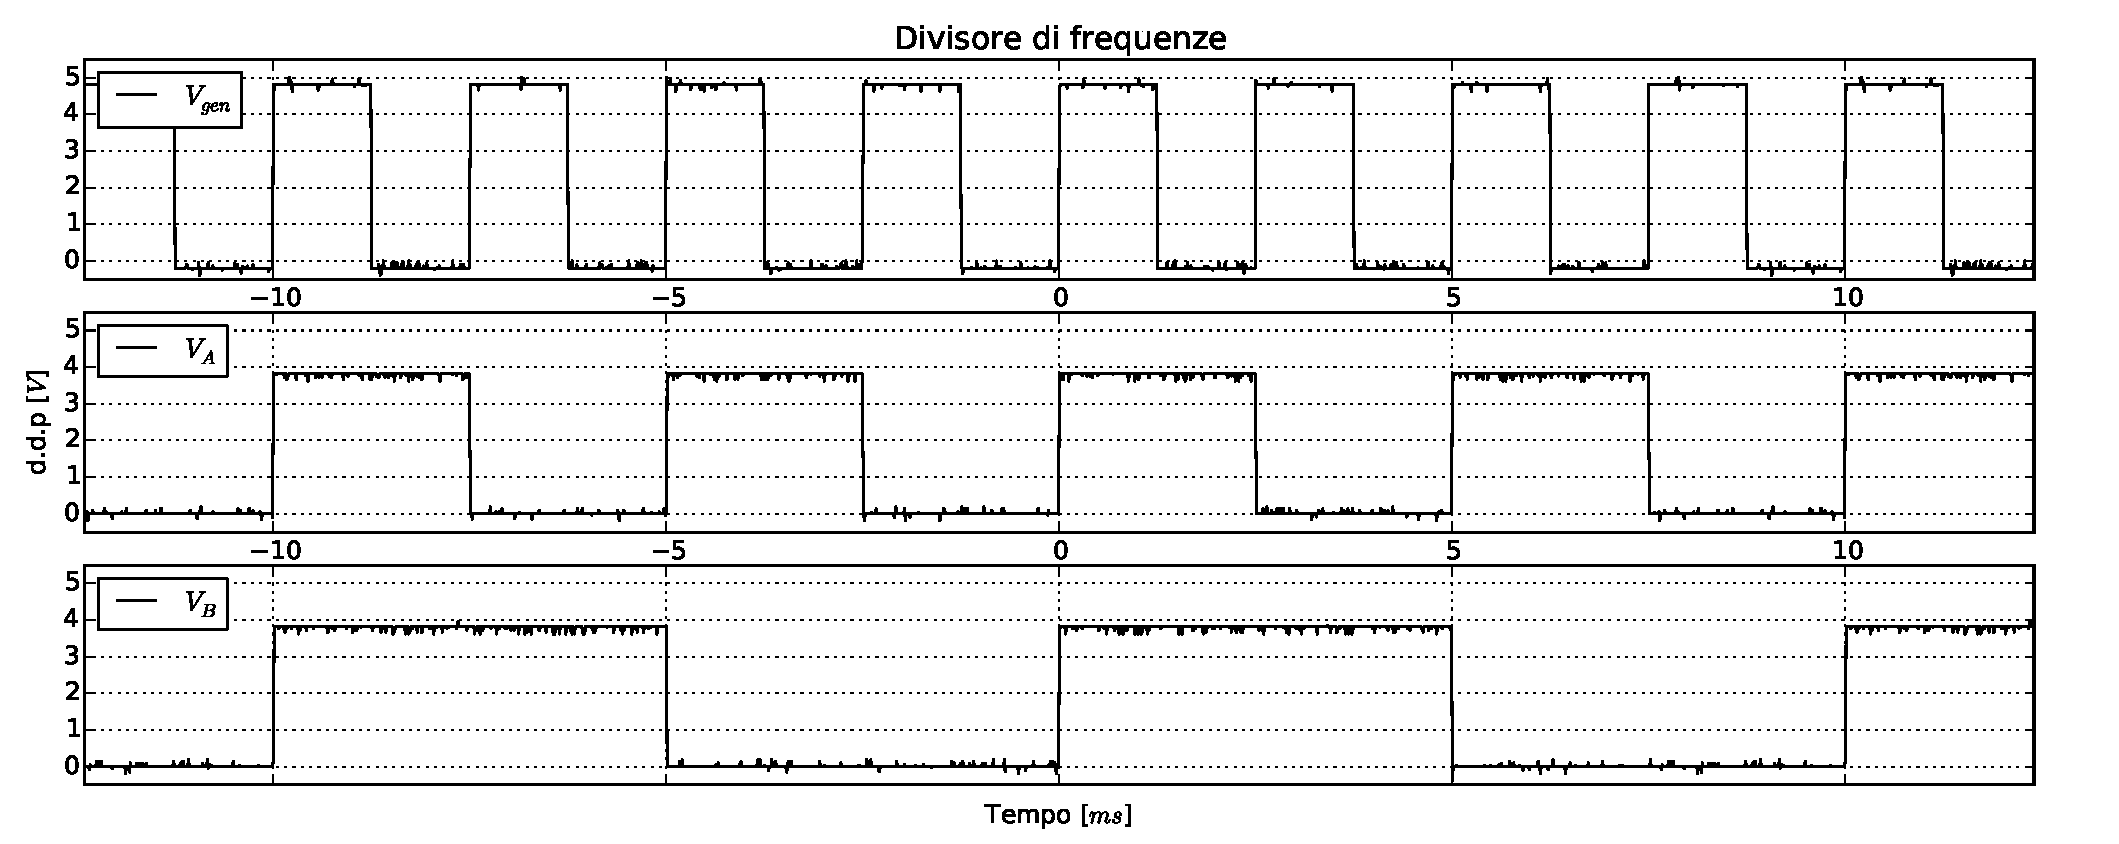
\includegraphics[width=.98\textwidth]{../E11/latex/gfreq.pdf}
	\caption{Risposta del divisore di frequenze da noi realizzato.}
	\label{gr11:freq}
\end{figure}


\subsection*{Conclusioni}


In questa esperienza abbiamo realizzato diversi circuiti a logica binaria utilizzando delle porte e dei Flip-Flop JK. Abbiamo implementato un circuito anti-rimbalzo e un divisore di frequenze.

%In questa esperienza abbiamo realizzato diversi circuiti logici partendo dalle porte logiche singole, ad esclusione del divisore di frequenze.
%In particolare abbiamo analizzato in funzionamento di diverse tipologie di Flip-Flop completando la tabella di verità.
%Inoltre abbiamo osservato il funzionamento di un interruttore con e senza un dispositivo di antirimbalzo, creato con porte logiche.
%Infine abbiamo realizzato un divisore di frequenze ponendo in serie due (o più) Flip-Flop di tipo JK.
